\begin{example}
Να υπολογιστεί ο πίνακας μετασχηματισμού της συμμετρικής απεικόνισης εικόνας ως προς άξονα \( w \) ο οποίος σχηματίζει γωνία \( \theta \) με τον θετικό άξονα των \( x. \)
\end{example}


\begin{figure}[h!]
	\begin{center}
		\begin{minipage}[b]{0.48\textwidth} % Top-left image
		    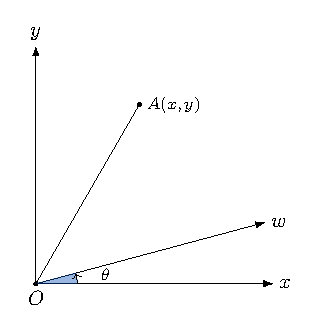
\includegraphics[width=\textwidth]{Chapter2/figure9a.pdf}
		\end{minipage}%
	\hfill
		\begin{minipage}[b]{0.48\textwidth} % Top-right image
		    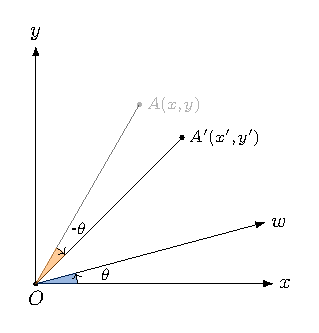
\includegraphics[width=\textwidth]{Chapter2/figure9b.pdf}
		\end{minipage}
	\end{center}
\caption{Παράδειγμα μεταφοράς σχήματος κατά διάνυσμα $v = (t_x, t_y)$}
\end{figure}


\begin{figure}[h!]
	\begin{center}
		\begin{minipage}[b]{0.48\textwidth} % Top-left image
		    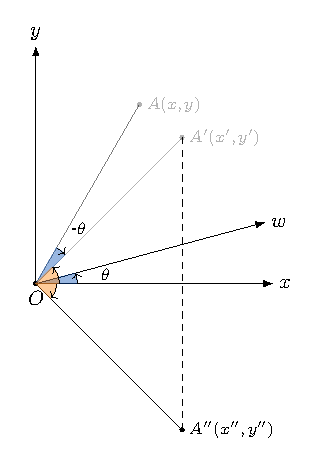
\includegraphics[width=\textwidth]{Chapter2/figure9c.pdf}
		\end{minipage}%
	\hfill
		\begin{minipage}[b]{0.48\textwidth} % Top-right image
		    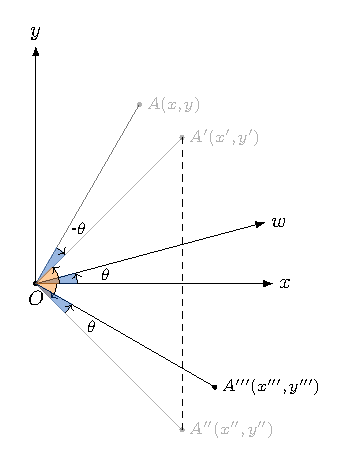
\includegraphics[width=\textwidth]{Chapter2/figure9d.pdf}
		\end{minipage}
	\end{center}
\caption{Παράδειγμα μεταφοράς σχήματος κατά διάνυσμα $v = (t_x, t_y)$}
\label{fig:9}
\end{figure}



Όπως φαίνεται και στο σχήμα \ref{fig:9} ο μετασχηματισμός μπορεί να προκύψει ως εξής:
 
\begin{tabular}{m{0.45\textwidth}m{0.5\textwidth}}
	1. Στροφή της εικόνας κατά γωνία \( -\theta \). & \( (R_{-\theta}) \) \\
	2. Συμμετρία ως προς άξονα $x$.& \( (M_x) \)\\
	3.  Στροφή της εικόνας κατά γωνία \( \theta \).& \( (R_{\theta}) \)
\end{tabular}


\[
\text{Βήμα 1: } 
\begin{bmatrix}
x' \\ y' \\ 1
\end{bmatrix}
=
\begin{bmatrix}
\cos(-\theta) & -\sin(-\theta) & 0 \\
\sin(-\theta) & \cos(-\theta) & 0 \\
0 & 0 & 1
\end{bmatrix}
\cdot
\begin{bmatrix}
x \\ y \\ 1
\end{bmatrix}
= \Pi_1
\begin{bmatrix}
x \\ y \\ 1
\end{bmatrix}
\]

\[
\text{Βήμα 2: } 
\begin{bmatrix}
x'' \\ y'' \\ 1
\end{bmatrix}
=
\begin{bmatrix}
1 & 0 & 0 \\
0 & -1 & 0 \\
0 & 0 & 1
\end{bmatrix}
\cdot
\begin{bmatrix}
x' \\ y' \\ 1
\end{bmatrix}
= \Pi_2
\begin{bmatrix}
x' \\ y' \\ 1
\end{bmatrix}
\]

\[
\text{Βήμα 3: } 
\begin{bmatrix}
x''' \\ y''' \\ 1
\end{bmatrix}
=
\begin{bmatrix}
\cos \theta & -\sin \theta & 0 \\
\sin \theta & \cos \theta & 0 \\
0 & 0 & 1
\end{bmatrix}
\cdot
\begin{bmatrix}
x'' \\ y'' \\ 1
\end{bmatrix}
= \Pi_3
\begin{bmatrix}
x'' \\ y'' \\ 1
\end{bmatrix}
\]

Άρα τελικά:
\[
\begin{bmatrix}
x''' \\ y''' \\ 1
\end{bmatrix}
=
\Pi_3 (\Pi_2 (\Pi_1
\begin{bmatrix}
x \\ y \\ 1
\end{bmatrix}))
\]

Επειδή ο πολλαπλασιασμός πινάκων είναι πράξη προσεταιριστική, θα έχουμε:

\[
\begin{bmatrix}
x''' \\ y''' \\ 1
\end{bmatrix}
=
(\Pi_3 \cdot \Pi_2 \cdot \Pi_1)
\begin{bmatrix}
x \\ y \\ 1
\end{bmatrix}
\]

και επομένως μπορούμε να υπολογίσουμε το γινόμενο $\Pi_3 \Pi_2 \Pi_1$ το οποίο θα αποτελεί και τον ζητούμενο πίνακα $\Pi$.

\[
\Pi =
\begin{bmatrix}
\cos \theta & -\sin \theta & 0 \\
\sin \theta & \cos \theta & 0 \\
0 & 0 & 1
\end{bmatrix}
\cdot
\begin{bmatrix}
1 & 0 & 0 \\
0 & -1 & 0 \\
0 & 0 & 1
\end{bmatrix}
\cdot
\begin{bmatrix}
\cos(-\theta) & -\sin(-\theta) & 0 \\
\sin(-\theta) & \cos(-\theta) & 0 \\
0 & 0 & 1
\end{bmatrix}
\]

\[
=
\begin{bmatrix}
\cos \theta & \sin \theta & 0 \\
-\sin \theta & \cos \theta & 0 \\
0 & 0 & 1
\end{bmatrix}
\cdot
\begin{bmatrix}
\cos \theta & \sin \theta & 0 \\
-\sin \theta & \cos \theta & 0 \\
0 & 0 & 1
\end{bmatrix}
=
\]

\[
\begin{bmatrix}
\cos^2\theta - \sin^2\theta & 2\sin\theta\cos\theta & 0 \\
2\sin\theta\cos\theta & \sin^2\theta - \cos^2\theta & 0 \\
0 & 0 & 1
\end{bmatrix}
\cdot
\begin{bmatrix}
\cos 2\theta & \sin 2\theta & 0 \\
\sin 2\theta & -\cos 2\theta & 0 \\
0 & 0 & 1
\end{bmatrix}
\]